\documentclass{beamer}
\usepackage{listings}
\lstset{
%language=C,
frame=single, 
breaklines=true,
columns=fullflexible
}
\usepackage{blkarray}
\usepackage{subcaption}
\usepackage{url}
\usepackage{tikz}
\usepackage{tkz-euclide} % loads  TikZ and tkz-base
%\usetkzobj{all}
\usetikzlibrary{calc,math}
\usepackage{float}
\newcommand\norm[1]{\left\lVert#1\right\rVert}
\renewcommand{\vec}[1]{\mathbf{#1}}
\usepackage[export]{adjustbox}
\usepackage[utf8]{inputenc}
\usepackage{amsmath}
\usepackage{tikz}
\usepackage{hyperref}
\usepackage{bm}
\hypersetup{
    colorlinks = true,
    linkbordercolor = {white},
    linkcolor={red},
    citecolor={green},
    filecolor={blue},
	menucolor={red},
	runcolor={cyan},
	urlcolor={blue},
	breaklinks=true
}
\usetikzlibrary{automata, positioning}
\usetheme{Boadilla}
\providecommand{\pr}[1]{\ensuremath{\Pr\left(#1\right)}}
\providecommand{\mbf}{\mathbf}
\providecommand{\qfunc}[1]{\ensuremath{Q\left(#1\right)}}
\providecommand{\sbrak}[1]{\ensuremath{{}\left[#1\right]}}
\providecommand{\lsbrak}[1]{\ensuremath{{}\left[#1\right.}}
\providecommand{\rsbrak}[1]{\ensuremath{{}\left.#1\right]}}
\providecommand{\brak}[1]{\ensuremath{\left(#1\right)}}
\providecommand{\lbrak}[1]{\ensuremath{\left(#1\right.}}
\providecommand{\rbrak}[1]{\ensuremath{\left.#1\right)}}
\providecommand{\cbrak}[1]{\ensuremath{\left\{#1\right\}}}
\providecommand{\lcbrak}[1]{\ensuremath{\left\{#1\right.}}
\providecommand{\rcbrak}[1]{\ensuremath{\left.#1\right\}}}
\providecommand{\abs}[1]{\vert#1\vert}

\makeatletter
\newenvironment<>{proofs}[1][\proofname]{%
    \par
    \def\insertproofname{#1\@addpunct{.}}%
    \usebeamertemplate{proof begin}#2}
  {\usebeamertemplate{proof end}}
\makeatother

\title{CSIR-UGC NET-June 2015-Question-110}
\author{Avula Mohana Durga Dinesh Reddy}
\date{CS20BTECH11005}
\begin{document}

\begin{frame}
\titlepage
\end{frame}

\begin{frame}
\frametitle{Question}
\begin{block}{CSIR-UGC NET-June 2015-Question-110}
Suppose X has density $f\brak{\frac{x}{\theta}}=\frac{1}{\theta} e^{-x/\theta},x>0$ where $\theta > 0$ is unknown.Define Y as follows:
\begin{align}
Y=k \text{ if } k \leq X < k+1, k=0,1,2 \cdots
\end{align}
Then the distribution of Y is :
\begin{enumerate}
\item Normal 
\item Binomial 
\item Poisson 
\item Geometric
\end{enumerate}
\end{block}
\end{frame}

\begin{frame}
\frametitle{Definitions}
\begin{block}{Definition of Normal Distribution}
The distributions which have probability distribution function in the form of 
\begin{align}
f\brak{x}=\frac{1}{\sigma \sqrt{2\pi}}e^{- \frac{1}{2} \brak{\frac{x-\mu}{\sigma}}^2}
\end{align} are known as normal distribution.\\
Where $\mu$ is mean(and also median and mode) and $\sigma$ is standard distribution of \textit{PDF}.
\end{block}
\begin{block}{Other Properties of Normal Distribution}
\begin{enumerate}
\item Normal distribution is also known as Gauss or Gaussian or Laplace-Gauss distribution.
\item It is a symmetric distribution function about its mean.
\end{enumerate}
\end{block}
\end{frame}

\begin{frame}
\frametitle{Definitions Contd.}
\begin{block}{Binomial Distribution}
Binomial distribution is a common probability distribution that models the probability of obtaining one of two outcomes under a given number of parameters.It's probability distribution function is in the form of 
\begin{align}
f\brak{k,n,p}=\pr{k,n,p}=\pr{X=k}= {n\choose k} p^k \brak{1-p}^{n-k}
\end{align}
Where 
\begin{itemize}
\item k is the number of occurences.
\item p is the probability of an outcome being true
\item n is total number of trials
\end{itemize}
\end{block}
\end{frame}

\begin{frame}
\frametitle{Definitions Contd.}
\begin{block}{Poisson distribution}
A random variable X is said to have poisson distribution with parameter $\lambda > 0$ ,if it has probability distribution function in the form of 
\begin{align}
f\brak{k,\lambda}=\pr{k,\lambda}=\frac{\lambda ^k e^{- \lambda}}{k!}
\end{align}
Where 
\begin{itemize}
\item k is the number of occurences\brak{k=0,1,2..}.
\item e is the eulers number.\brak{e=2.71828}
\end{itemize}
\end{block}
\end{frame}

\begin{frame}{Definitions Contd.}
\begin{block}{Geometric distribiution}
A distribution is said to be a geometric distribution if it is one of the two following distributions
\begin{enumerate}
\item The probability distribution of X number of bernoulli trials needed to get one success, supported on the set \brak{1,2,3..}
\begin{align}
\pr{X=k}=\brak{1-p}^{k-1} p , \brak{k=1,2,3,\cdots}
\end{align}
\item The probability distribution of number Y=X-1 of failures before the first success, supported on the set \brak{0,1,2,3..}
\begin{align}
\pr{Y=k}=\pr{X=k+1}=\brak{1-p}^k p , \brak{k=0,1,2,\cdots}
\end{align}
\end{enumerate}
\end{block}
\end{frame}

\begin{frame}{Solution}
\begin{lemma}
PDF of X is 
\begin{align}
P\brak{X=x}&=e^{-x}
\end{align}
\end{lemma}
\begin{proofs}
Given \textit{PDF} of X is 
\begin{align}
f\brak{\frac{x}{\theta}}&=\frac{1}{\theta} e^{-x/\theta},x>0,\text{where } \theta >0 \text{ is unknown}\\
f\brak{X}&=\frac{1}{\theta}e^{-X},X>0\text{ as }x>0,\theta>0
\end{align}
\end{proofs}
\end{frame}

\begin{frame}{Solution Contd.}
\begin{proof}[\proofname\ (Contd.)]
$\because$ The total probability is 1 
\begin{align}
\int_0 ^\infty f\brak{X} dX &=1 \\
\int _0^\infty \frac{1}{\theta} e^{-X} dX&=1 \nonumber \\
\frac{1}{\theta}&=1 \nonumber \\
\Rightarrow \theta &=1 \\
\text{So }f\brak{X} = e^{-X}
\end{align}
Hence lemma 2.2 is proved.
\end{proof}
\end{frame}

\begin{frame}{Solution Contd.}
\begin{lemma}
PDF of Y is 
\begin{align}
p\brak{Y=k}&=e^{-k} \brak{1-e^{-1}}
\end{align}
and is in the form of geometric distribution.
\end{lemma}
\begin{proof}
Also given that Y=k if $k \leq X <k+1$ k=0,1,2,$\cdots$
\begin{align}
p\brak{Y=k}&=\int_k^{k+1} p\brak{X=x} dx\\
&=\int_k^{k+1} e^{-x} dx \nonumber \\
&=e^{-k}\brak{1-e^{-1}} \label{PDF of Y}
\end{align}
Hence using lemma 2.1  and (\ref{PDF of Y}) lemma 2.3 is proved.
\end{proof}`
\end{frame}

\begin{frame}{Example figure}
\begin{figure}[ht]
    \centering
    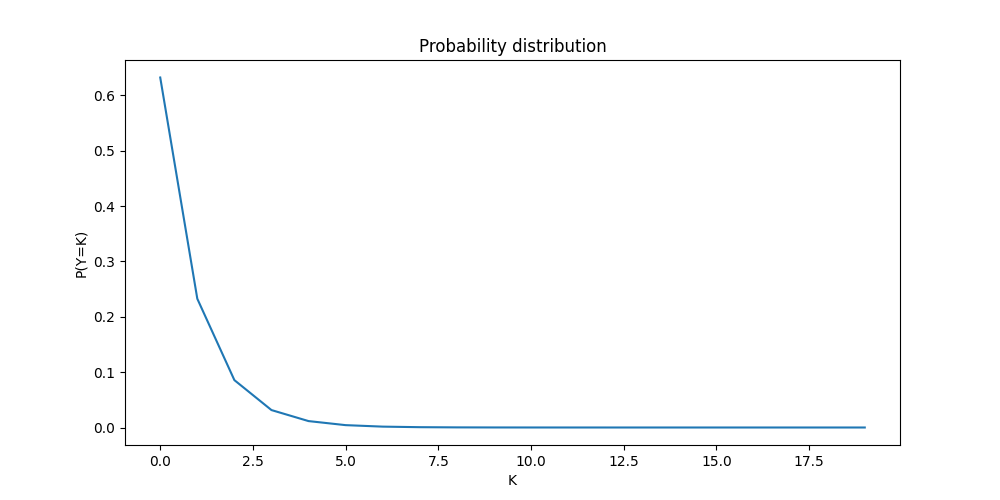
\includegraphics[width=1\textwidth]{Figure_1.png}
    \caption{Probability distribution of Y}
    \label{fig:my_label}
\end{figure}
\end{frame}
\end{document}